%%%%%%%%%% FILE sec/0_abstract.tex
\begin{abstract}
A vision-based tactile sensor (VBTS), such as the GelSight, images the deformation of a soft gel with an internal camera. Its fine detail lets robots recognise the material they touch, and learned models treat its images as pictures of the touched surface. We find that every image also contains a faint pattern and an uneven illumination that belong to the sensor itself. Over four months of robot grasps of 20 materials with two GelSight Mini units and three gels, this hardware state drifted only slightly with use and changed abruptly whenever the unit or the gel was replaced. Because tactile datasets often record each object in its own session, a material classifier can learn the state as part of each material. After a change of hardware, it then mistakes other materials for the few that the new hardware recorded in training. In a public dataset of four GelSight Minis, training one object only on the test sensor halves the accuracy on the other objects tested on that sensor. We read touch together with the sensor's state, using only the robot's own unlabelled contacts. At test time, every image is read relative to a running estimate of the state, which needs no training. A retrained encoder is also aligned with the contacts recorded after the change. On 55 sessions recorded on hardware on which their material was not learned, the reading alone raises a ResNet-50 from 32.4 to 44.8\pct\ (chance 5\pct), as much as the best of five test-time adaptation methods. It also improves every domain adaptation method we add it to, and with alignment the ResNet-50 reaches 61.6\pct.
\end{abstract}

%%%%%%%%%% FILE sec/1_intro.tex
\section{Introduction}
\label{sec:intro}

A vision-based tactile sensor (VBTS) presses a soft elastomer gel onto a surface and photographs the gel's deformation with a camera behind it~\cite{yuan2017gelsight,dong2017improved,lambeta2020digit}. One touch thus records the shape of the contact, the forces on it and the texture of the surface at a resolution of tens of micrometres, and inexpensive units such as the GelSight Mini and DIGIT have made the sensor common on robot grippers. Robots use these images to predict whether a grasp will hold~\cite{calandra2017feeling}, to detect slip~\cite{dong2017improved}, to slide a cable through their fingers~\cite{she2021cable}, to reconstruct and rotate objects in the hand~\cite{suresh2024neuralfeels,qi2023rotateit} and to recognise what they touch~\cite{li2013texture,yuan2017connecting,yang2022touchandgo}. Because the output is an image, the models come from computer vision, and encoders pretrained on millions of tactile frames now serve all of these tasks~\cite{higuera2024sparsh,t3fota2024,unitouch2024,anytouch2025}.

This paper studies one of these tasks, recognising the material of a surface from a single grasp. The material tells a robot how a surface will slip, how hard it may be squeezed and where an object should be sorted, and material recognition is a standard benchmark for tactile encoders~\cite{higuera2024sparsh,unitouch2024,anytouch2025}. It is also the task most exposed to the problem we describe. The shape of a contact changes the image strongly, but what separates one material from another is faint, fine detail, and the sensor adds faint, fine detail of its own. A robot keeps its sensors for months. Over that time the sensor is powered off and on, and its gel is lubricated and worn. Eventually the gel, a consumable part, is replaced, and so is a unit that fails~\cite{davis2025resilience,cottrell2026durable}. If a classifier depends on the hardware, such routine maintenance breaks it, and the robot has no labels with which to notice.

\begin{figure}[t]
  \centering
  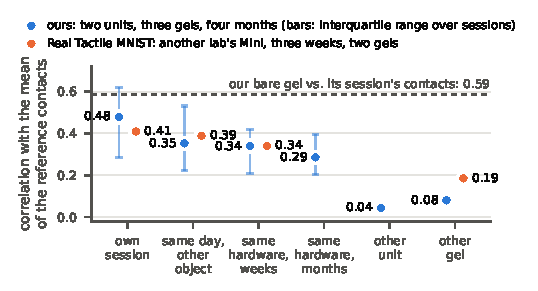
\includegraphics[width=\linewidth]{fig/fig_day_signature.pdf}
  \caption{\textbf{The hardware is in every image.} Correlation between the fine detail (190--370\,\si{\micro\metre}) of a contact image and the position-wise mean of other contacts, grouped by how the other contacts relate to it. Pixels within 60\,px of a printed marker are excluded. Blue: our recordings (55 sessions, two units, three gels, four months). Orange: another lab's GelSight Mini (Real Tactile MNIST~\cite{tactilemnist2025}, three weeks, two gels). Dashed: our bare-gel frames against their session's mean contact frame.}
  \label{fig:signature}
\end{figure}

An image is formed by the camera, the LEDs and the gel cartridge as well as by the object. These parts leave a faint imprint of their own in every image. We call this part of the image the sensor's \emph{hardware state}. It has two parts, a fine pattern carried by the gel cartridge and a smooth, uneven illumination. We recorded 2,711 grasps of 20 materials over four months with two GelSight Mini units and three gels, and \cref{fig:signature} shows how strong the fine pattern is in them. At a fixed image position, the fine detail of a contact correlates at 0.34 with other objects pressed on the same unit and gel weeks later and at 0.29 three months later, but only at 0.04 and 0.08 with a different unit or gel. The images alone show when the hardware changed, and they corrected our laboratory log. A model that classifies touch also sees the hardware, and this paper asks what it does with it.

That the sensor appears in the image is known, and three practices deal with it. The first subtracts a frame of the unloaded gel, captured once or at intervals~\cite{gelslim2018,tactic2026,higuera2024sparsh,sitr2025,anytouch2026two,htt2026}. The second diversifies the training data across units and optics~\cite{suresh2024neuralfeels,tactic2026,sitr2025}. The third avoids raw appearance, for example by reading marker displacements, which survive ``damage or gel replacements''~\cite{rdp2025}. The evaluations behind these practices use one collection, or several units recorded at about the same time~\cite{sitr2025,bideta2026,feats2025,tacverse2026,rct2026,anytouch2026two}, and the longest span we found is three weeks~\cite{tactilemnist2025}. We found no study that follows one unit and gel for months or measures what the blank frame removes, and none that asks what a change of hardware does to a classifier. Medical imaging has asked this question. A network trained to find pneumonia in chest X-rays from several hospitals also learned which hospital had taken each X-ray. Pneumonia was far more common at one of them, so the hospital helped its predictions, and its accuracy fell at hospitals it had not seen~\cite{zech2018hospital}.

Why would a classifier use the hardware? Many tactile datasets record each object in its own session, and in ours each material was learned on one hardware configuration. Every training image of a material therefore carries two cues, the texture of the material and the imprint of the hardware it was recorded on. The imprint tells the classifier which group of materials an image can belong to. In June and July, unit 2 had recorded only four of the 20 materials, so for a classifier trained on those months, the imprint of unit 2 means ``one of those four''. Everything in September and October was recorded on unit 2. A ResNet-50 trained on June and July assigns 64\pct\ of these test episodes to the four materials, and it recognises the sixteen materials that it learned on unit 1 at only 35\pct, where chance is 5\pct. Frozen Sparsh encoders~\cite{higuera2024sparsh} fail in the same way (supplement).

To confirm that the imprint causes this failure, we create the same situation in a dataset that does not have it. SITR~\cite{sitr2025} pressed the same 20 objects on four GelSight Minis. We train on 19 objects pressed on one Mini and on one object pressed only on a second Mini, and we test all objects on the second Mini. Only one training object then carries the imprint of the second Mini, and 62\pct\ of the test images are assigned to it. Accuracy on the objects learned on the first Mini falls from 73.9\pct, when no object is tied to the second Mini, to 37.0\pct.

The cure is to read touch together with the state of the sensor, and a robot can do this with its own stream of contacts. Our method has two parts. At test time, the robot averages the contacts it has made since the hardware last changed into a running estimate of the state, as microscopy estimates a flat-field from its own images~\cite{singh2014illumination,peng2017basic}. It subtracts the smooth illumination part of that estimate from every image (\cref{alg:tracker}). A detector dates the changes of hardware from whole frames, so that the estimate restarts when the unit or the gel is replaced. This reading needs no labels and no training, so it can be added to any classifier. If the encoder can be retrained, the same stream serves as the target domain of a conditional adversary from domain adaptation~\cite{long2018cdan}, so that the encoder's features stop separating the old hardware from the new. This alignment also reaches the fine pattern, which the reading leaves in place.

We evaluate on 55 sessions, each recorded on hardware other than the one its material was learned on. The reading alone raises a ResNet-50 from 32.4 to 44.8\pct. That matches the best of five published test-time adaptation methods on the robot's stream, where four of them collapse because each batch holds a single material. Added to published domain adaptation methods, the reading improves every one of them, and with alignment the ResNet-50 reaches 61.6\pct. The gains hold for a CNN trained from scratch and for ConvNeXt and DINOv2 encoders. The reading removes only an additive state. SITR's Minis also differ in their field of view and contrast, and there the reading does not help, but alignment does.

Our contributions are:
\begin{itemize}\setlength{\itemsep}{1pt}
  \item A four-month measurement of the hardware state of a VBTS. The state is present in the bare gel, stable with use and replaced with the unit or the gel.
  \item Evidence that material classifiers trained with one object per session use this state as a shortcut, on our recordings and, under control, on a public dataset.
  \item A method that reads touch relative to the state using only the robot's unlabelled contacts, compared with ten adaptation methods and four encoders, with its limits shown.
  \item A four-month VBTS dataset with two units, three gels, 20 materials, co-recorded force and bare-gel frames, which we release with a cross-hardware protocol and the code.
\end{itemize}

%%%%%%%%%% FILE sec/2_related.tex
\section{Related work}
\label{sec:related}

\paragraph{Tactile representations and their evaluation.}
Self-supervised tactile encoders are trained on large frame collections: Sparsh~\cite{higuera2024sparsh}, T3~\cite{t3fota2024}, UniTouch~\cite{unitouch2024}, AnyTouch~\cite{anytouch2025,anytouch2026two} and the TVL data~\cite{tvl2024}. TactSpace aligns several views of one contact in a shared latent space~\cite{tactspace2026}. These models are evaluated inside the collection they were trained on, with random or object-level splits. RCT shows that frame-level splits of TVL leak the sequence and that a held-out DIGIT is a separate difficulty~\cite{rct2026}, and a recent material benchmark on TVL's HCT data still shares sessions between training and test~\cite{mohsan2026language}. The sensor enters as preprocessing: Sparsh, SITR, AnyTouch~2 and HTT subtract a background frame~\cite{higuera2024sparsh,sitr2025,anytouch2026two,htt2026}, and UniTouch adds a token for the sensor type~\cite{unitouch2024}. GelSlim re-captures its blank frame every hundred grasps~\cite{gelslim2018}, and other work measures how the unloaded image degrades with use~\cite{davis2025resilience,cottrell2026durable}. None of these studies holds out hardware of the same model over months or tests what the background frame removes.

\paragraph{Transfer across units and gels.}
That units of one model differ is well documented. SITR combines background subtraction, 18 calibration presses per unit and a million simulated images, and reaches 90\pct\ when a 16-object classifier is moved between four GelSight Minis, against 73\pct\ for an ImageNet ViT~\cite{sitr2025}. BIDETA adapts frozen Sparsh to sibling units with labelled target contacts~\cite{bideta2026}. TacVerse benchmarks seven sensors with chronological splits inside one campaign~\cite{tacverse2026}. FEATS and FeelAnyForce find that force estimates degrade on a new unit or gel~\cite{feats2025,feelanyforce2024}. Others translate between sensors conditioned on the target's blank frame~\cite{genforce2026,castano2026forcemap,split2026} or align different sensor types~\cite{cttp2024,htt2026}. Each of these methods needs blank frames, calibration presses, simulation or target labels. Our estimate needs only the robot's ordinary contacts.

\paragraph{Domain adaptation and test-time adaptation.}
Adapting a classifier to a shifted test distribution without labels is the subject of unsupervised domain adaptation. Retraining methods align the features of labelled source data and unlabelled target data with a domain adversary~\cite{ganin2016dann}, conditioned on the classifier's predictions in CDAN~\cite{long2018cdan}, reduce the confusion between classes on the target~\cite{jin2020mcc}, smooth the loss landscape~\cite{rangwani2022sdat} or enforce consistency under masking~\cite{hoyer2023mic}. Under a standardised setup, newer methods often do no better than CDAN~\cite{kalluri2024udabench}. Test-time methods adapt a trained model on the test stream instead, by re-estimating normalisation statistics~\cite{li2018adabn}, by minimising the entropy of the predictions~\cite{wang2021tent,niu2023sar,lee2024deyo}, or by averaging predictions over augmented copies of an input~\cite{zhang2022memo}. Most assume batches that mix classes. When the stream is ordered by object, as a robot's stream is, normalisation statistics absorb the object~\cite{burns2021bn}, and dedicated methods handle temporal correlation~\cite{gong2022note,boudiaf2022lame,yuan2023rotta}. Other methods add a signal from the structure of a new problem, such as the correspondence of RGB and flow~\cite{munro2020mmsada}, or remove a domain gap caused by sensor hardware, as Complete \& Label does for LiDAR beam patterns~\cite{yi2021completelabel}. Low spatial frequencies carry much of a camera's and an illuminant's style, which FDA swaps between domains~\cite{fda2020}. Our reading removes the smooth part of a state estimated from the robot's own stream instead, and our alignment uses that stream as the target domain. The detector that dates changes is a two-window test in the tradition of sequential change detection~\cite{page1954cusum}.

\paragraph{Acquisition shortcuts and flat-fields from the data.}
Classifiers that learn the hospital from a radiograph~\cite{zech2018hospital}, the acquisition setup from a COVID study~\cite{degrave2021covid} or the dataset from a photograph~\cite{torralba2011bias,liuhe2025} are instances of shortcut learning~\cite{geirhos2020shortcut}, and our finding is the tactile instance. Removing batch information by gradient reversal does not improve generalisation to unseen batches there~\cite{sypetkowski2023rxrx1}. Our alignment instead uses unlabelled images from the new hardware itself. Multi-site MRI removes each scanner's additive and multiplicative effect from its measurements~\cite{fortin2017combat}. Microscopy estimates an illumination field from the image collection itself, as the per-pixel mean of a batch~\cite{singh2014illumination} or its low-rank refinement~\cite{peng2017basic}, and infrared imaging does the same for fixed-pattern noise~\cite{harris1999nuc}. The same averaging identifies a camera by its sensor noise~\cite{lukas2006prnu}. Our estimate is such a flat-field, taken from a robot's stream of contacts and restarted when the hardware changes.

%%%%%%%%%% FILE sec/3_signature.tex
\section{The hardware state in a tactile image}
\label{sec:signature}

\paragraph{Data.}
A GelSight Mini (1640$\times$1232 native frames, \SI{11.3}{\micro\metre}/px, \SI{18.8}{fps}, printed markers) is mounted on one finger of a parallel gripper, and an ATI Nano17 on the other finger measures the normal force. The object is a box whose face carries one of 20 materials. It is clamped in a fixture with foam behind it so that the contact aligns itself. Each episode grasps the face at one of two forces (40 or 80\pct\ of a per-material maximum, 0.9--5\,N) and strokes it by 2\,cm in four directions and a circle. The gel is lubricated every five episodes, and one session records one material. Four campaigns cover four months: A (June 15--22), B (July 6--8), C (July 9--13) and D (September 22 to October 15), 2,711 episodes in all. 10 episodes of campaign D have no eight-frame span of contact inside the stroke, so the material experiments use 2,701. Campaign D also records frames of the bare gel. The camera's exposure and white balance are fixed: on a held contact the mean of each colour channel drifts by at most 0.3 grey levels per episode. We never resample a frame.

Two units and three gels were used. Unit 1 carried gel 1 until July 9, unit 2 carried gel 2 from July 10, and gel 3 replaced gel 2 on October 9 between 18:42 and 19:37. We call these three combinations of unit and gel the hardware configurations S1, S2 and S3. The images themselves give these dates, as the end of this section shows.

\paragraph{Measurement.}
For every session we form the position-wise mean of its contact crops in frame coordinates, its \emph{mean contact frame} $M_s(p)$. For a sampled contact crop we correlate its fine band (190--370\,\si{\micro\metre}) with the same band of another session's mean frame, excluding pixels within 60\,px of a printed marker so that inpainting residue cannot contribute. \Cref{fig:signature} shows the medians over sessions. A contact matches the other contacts of its own session, which include the same object, at 0.48. It matches another object touched the same day at 0.35, the same unit and gel on another day at 0.34, and the same unit and gel three months later at 0.29. It does not match the other unit (0.04) or the other gel of the same unit (0.08). Frames of the bare gel, with nothing touching it, match their session's mean contact frame at 0.59. Another lab's GelSight Mini shows the same ordering~\cite{tactilemnist2025}, although its correlation across a gel swap stays higher (0.19).

\begin{figure}[t]
  \centering
  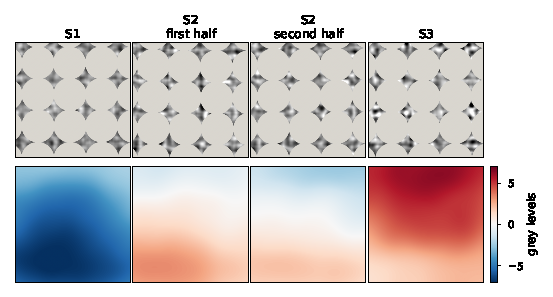
\includegraphics[width=\linewidth]{fig/fig_state_images.pdf}
  \caption{\textbf{What the hardware state looks like.} The mean contact frame of each hardware configuration (each session counted once) in one 4.7-mm region of the frame. Top: the fine band (190--370\,\si{\micro\metre}), with pixels within 60\,px of a printed marker greyed out. Bottom: the smooth illumination field relative to the mean of the four panels ($\pm$7 grey levels). The two halves of S2's sessions, different objects weeks apart, share a pattern that the other configurations do not.}
  \label{fig:stateimages}
\end{figure}

\paragraph{What the state is.}
\Cref{fig:stateimages} shows the two parts of the state. Two tests locate the fine pattern. It does not move with the membrane: warping a bare-gel frame by the membrane's measured displacement lowers its match to the session's mean frame from 0.59 to 0.54. The membrane moves by a median of only 2.1\,px, however, so this test is weak. The pattern does belong to the gel cartridge, because a new gel on the same unit and camera removes it. We therefore take it to be an optical property of the cartridge, fixed in the camera's view, rather than texture on the deforming surface. The smooth part, the illumination field, changes a little from session to session on the same hardware. Between two bare-gel frames of one session, the illumination moves by a median 0.13 grey levels over 5 grasps. Between the last bare-gel frame of one session and the first of the next, with no contact in between, it moves by 0.40. The illumination therefore moves more while the sensor rests between sessions than while it is used. Within one configuration, a session's illumination field lies 0.5--1.3 grey levels from the configuration's mean. The two units differ by 3.8 grey levels, and the two gels on unit 2 by 2.9.

\paragraph{The images record the hardware history.}
The changes are sharp enough to date from the images alone. Correlating every pair of the 35 June and July sessions splits them into two blocks at July 9 to 10 and nowhere else, and the September and October sessions split at October 9. Our laboratory log had recorded a change of unit and four gel replacements. The images show only the two changes above, and the operators confirmed them against their notes, so the timeline above is the one the images give. \Cref{sec:tracker} turns the same observation into a detector that runs while the robot works.

\begin{figure}[t]
  \centering
  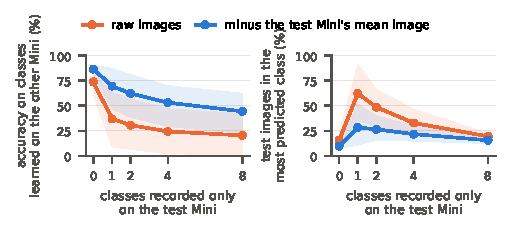
\includegraphics[width=\linewidth]{fig/fig_confound.pdf}
  \caption{\textbf{Tying classes to hardware, under control.} SITR~\cite{sitr2025} pressed 20 objects on four GelSight Minis. We train on $20-k$ classes recorded on one Mini and $k$ classes recorded only on the test Mini, and test all classes on the test Mini (frozen DINOv2, MLP head; mean over 12 Mini pairs and class draws, band: 10th--90th percentile over pairs).}
  \label{fig:confound}
\end{figure}

\paragraph{The state as a shortcut.}
\label{sec:confound}
In our training data each material appears under one hardware configuration, because each was recorded in its own session. A classifier can then use the state as a feature of the materials recorded under it. The introduction tests this by tying classes to one of SITR's four Minis~\cite{sitr2025}, and \cref{fig:confound} shows the test in full. A frozen DINOv2 with an MLP head is trained on $20-k$ objects pressed on one Mini and on $k$ objects pressed only on the test Mini, and the results are averaged over 12 pairs of Minis and draws of the tied objects. On Real Tactile MNIST~\cite{tactilemnist2025} we tie digits to gels instead. Tying one digit to the test gel sends 100\pct\ of the test touches to that digit.

%%%%%%%%%% FILE sec/4_method.tex
\section{Reading touch after a change of hardware}
\label{sec:method}
\label{sec:tracker}

\paragraph{Setting.}
A classifier is trained on labelled contacts recorded on some hardware configurations. Then the unit or the gel is replaced, and the robot keeps working. It has no labels for its new contacts, no calibration object and, in most archived data, no frame of the bare gel. What it does have is the stream of its own contacts with whatever it touches, all recorded under the new state. The method uses that stream twice: to read every test image relative to an estimate of the state (\cref{alg:tracker}), and as the target domain when the encoder is retrained.

\paragraph{The state in an image.}
We write a contact image at frame position $p$, taken on hardware configuration $h$, as $x(p) = F_h(p) + r(p)$: the state of that configuration plus the touch. \Cref{sec:signature} showed that $F_h$ is shared by every object imaged on that hardware and is replaced with the unit or the gel. It has two parts, a fine pattern and a smooth illumination field. Because each object in a typical dataset is recorded in its own session, and therefore on one configuration, a classifier can use $F_h$ as a feature of the classes recorded under it. After a change of hardware, every image then carries the feature of the wrong classes, as the injected tie on SITR shows (\cref{fig:confound}).

\begin{algorithm}[t]
\caption{Reading the robot's stream relative to its hardware state}
\label{alg:tracker}
\begin{algorithmic}[1]
\Require training mean $G$; Gaussian low-pass $L_\sigma$; change detector with thresholds from the training data
\State $\mathcal S \gets \emptyset$ \Comment{mean contact frames of the sessions since the last change}
\For{each session of the stream (one object, no label)}
  \State $\hat F \gets \big(G + \sum_{M\in\mathcal S} M\big) / \big(1 + |\mathcal S|\big)$
  \For{each episode of the session}
    \State \textbf{read} every contact crop: $x'(p) \gets x(p) - L_\sigma\big(\hat F - G\big)(p)$ \Comment{to the encoder}
    \If{the detector declares a change of hardware}
      \State $\mathcal S \gets \emptyset$; \ $\hat F \gets G$
    \EndIf
  \EndFor
  \State add the session's mean contact frame to $\mathcal S$
\EndFor
\end{algorithmic}
\end{algorithm}

\paragraph{Reading relative to the state.}
The robot estimates the current state as the mean of the contact frames it has recorded since the last change of hardware. Each earlier session contributes its mean contact frame, so every object counts once. The training mean $G$, the average of the training sessions' mean contact frames, counts as one more session. The estimate is causal. A session is read with the estimate built from the sessions before it, so the first session after a change is read relative to $G$ alone, which leaves it unchanged. Every object imprints the gel differently, so averaging over objects leaves the hardware. This is the retrospective flat-field of microscopy~\cite{singh2014illumination,peng2017basic}, taken from a robot's stream.

The reading subtracts only the smooth part of the difference between the estimate and the training mean, a Gaussian low-pass with $\sigma = 33$\,px (0.37\,mm). There are two reasons. An estimate built from a few objects still contains their average imprint, and that imprint lies mostly in the fine band. The smooth illumination field, on the other hand, is estimated well from a few objects, and it carries most of the difference between hardware states: our two units differ by 3.8 grey levels in it. The reading needs no labels, no training and no bare-gel frame. It changes the input of a trained classifier, so it can be added to any classifier, including one trained with a published adaptation method (\cref{sec:baselines}). Only the test images are read. The training images and the stream used for alignment enter as recorded (row h of \cref{tab:ablation} reads the training images as well).

\paragraph{Dating the changes.}
The estimate must restart when the hardware changes, and a robot is not always told when that happens. The detector therefore watches whole frames, which the robot records anyway. It compares the mean frame of the last $K\!=\!8$ episodes with that of the $W\!=\!30$ episodes before them in two statistics. The first is the correlation of their fine bands (190--370\,\si{\micro\metre}, at least 60\,px from any marker), which drops when the cartridge's pattern changes. The second is the mean absolute difference of their illumination fields (Gaussian, $\sigma\!=\!33$\,px). Either alone raises false alarms, because a strongly textured material lowers the fine-band correlation on any hardware and the illumination moves a little between sessions. A change is declared only when both leave the same-hardware range for $m\!=\!5$ consecutive episodes. The thresholds are the 10th percentile of the correlation and the 95th percentile of the illumination distance on the first training configuration. \Cref{sec:trackerexp} evaluates the detector.

\paragraph{Aligning the encoder with the robot's own touches.}
The reading removes an additive, smooth state. The fine pattern remains, and two sensors can also differ in ways that are not additive, such as the part of the gel the camera sees or the contrast of the image (\cref{sec:second}). For these, the encoder must stop separating the old hardware from the new. When the encoder is retrained, we give it the unlabelled stream from the new hardware as the target domain of an adversarial alignment. We use CDAN+E~\cite{long2018cdan} unchanged. With the reading, it gave the highest accuracy of the aligners we tried, although DANN, SDAT and MIC come within the interval (\cref{sec:baselines}). A domain discriminator receives the outer product of the encoder's features and the classifier's detached predictions. When this product has more than 4096 dimensions, it is randomly projected to 1024. Each sample is weighted by $1 + e^{-H(\hat y)}$, so that confident predictions count more, and the encoder is trained against the discriminator through gradient reversal with a warm-start schedule. The objective is the cross-entropy on the labelled training crops plus the discriminator's weighted loss, with weight one, as in the Transfer-Learning-Library implementation.

%%%%%%%%%% FILE sec/5_experiments.tex
\section{Experiments}
\label{sec:exp}

\paragraph{Protocol.}
We test every recording of a material made on hardware other than the one it was learned on. Three folds hold out campaign D (September and October), campaign C (July 9--13), and campaigns A and B together (June and early July), and each trains on the remaining campaigns. Across the three folds this gives 55 test sessions, each tested once. In 47 of them the material was learned on the other unit, and in 8 on the other gel of the same unit. For the fold that holds out A and B, which trains on later campaigns and tests on earlier ones, we wrote down our predictions before training any model (supplement). Each session holds one material. We report the share of a session's episodes that are classified correctly, averaged over the 55 sessions, with 95\pct\ intervals from a bootstrap over sessions and paired bootstrap intervals for differences between methods. Chance is 5\pct. We also report the share of test episodes assigned to the most predicted class, averaged over the folds, which exposes a collapse onto few classes.

\paragraph{Training and the stream.}
Unless stated otherwise, every method uses the same encoder, a ResNet-50~\cite{he2016resnet} that starts from its ImageNet weights and is fine-tuned at the native \SI{11.3}{\micro\metre}/px on 192-px crops along the contact, with flips, quarter turns and photometric jitter. We call this training the recipe. An episode is classified by the mean log-probability of 24 crops, from three positions along the contact and eight frames of the stroke. Table rows average three training seeds, and the comparisons between the closest methods use five. Every method that adapts receives the same unlabelled stream: all contacts recorded on the test hardware in the test campaign. The stream therefore contains the test sessions themselves, as a working robot's stream would, and row~i of \cref{tab:ablation} scores sessions that the stream never contained. Every method is given the true dates of the changes, so that the reading and the test-time baselines, which are reset at each change, use the same knowledge. \Cref{sec:trackerexp} replaces the true dates with the detector's alarms.

\begin{table}[t]
  \centering\footnotesize\setlength{\tabcolsep}{3pt}
  \caption{\textbf{Comparison with published adaptation methods} on the 55 cross-hardware sessions (episode accuracy, three seeds, chance 5\pct). Unit / gel: the 47 sessions whose material was learned on the other unit and the 8 learned on the other gel. Top: share of test episodes in the most predicted class, averaged over the folds. Test-time methods adapt the trained recipe model on the robot's stream in recording order and are reset at each change of hardware. Retraining methods use the same stream without labels during training. $+$\,reading: test images read with \cref{alg:tracker}.}
  \label{tab:baselines}
  \resizebox{\linewidth}{!}{%
  \begin{tabular}{@{}lcccc@{}}
    \toprule
    method & all [95\pct\ interval] & unit (47) & gel (8) & top \\
    \midrule
    recipe, no adaptation & 32.4 [22.5, 42.1] & 29.0 & 52.2 & 33 \\
    \midrule
    \multicolumn{5}{@{}l}{\emph{test time, on the stream, no retraining}} \\
    test-time BatchNorm~\cite{li2018adabn} & 10.5 [7.0, 14.6] & 11.9 & 2.2 & 28 \\
    Tent~\cite{wang2021tent} & 10.6 [7.0, 14.7] & 12.0 & 2.1 & 28 \\
    SAR~\cite{niu2023sar} & 10.5 [7.0, 14.6] & 11.9 & 2.1 & 28 \\
    DeYO~\cite{lee2024deyo} & 10.6 [7.0, 14.7] & 12.0 & 2.0 & 28 \\
    RoTTA~\cite{yuan2023rotta} & 41.7 [32.5, 50.9] & 45.7 & 18.2 & 18 \\
    reading (\cref{alg:tracker}), ours & \textbf{44.8}\ [34.7, 54.8] & 44.1 & 48.9 & 19 \\
    \midrule
    \multicolumn{5}{@{}l}{\emph{retraining with the unlabelled stream}} \\
    DANN~\cite{ganin2016dann} & 53.4 [43.2, 62.4] & 54.2 & 48.3 & 20 \\
    \ \ $+$ reading & 60.6 [50.9, 70.0] & 64.4 & 38.2 & 15 \\
    MCC~\cite{jin2020mcc} & 42.7 [33.8, 51.7] & 43.3 & 39.0 & 20 \\
    \ \ $+$ reading & 45.9 [36.6, 55.1] & 48.7 & 29.8 & 19 \\
    SDAT~\cite{rangwani2022sdat} & 48.6 [38.2, 58.1] & 49.8 & 41.1 & 26 \\
    \ \ $+$ reading & 58.8 [48.7, 68.4] & 62.6 & 36.4 & 17 \\
    MIC~\cite{hoyer2023mic} & 55.3 [44.9, 65.4] & 60.0 & 28.2 & 22 \\
    \ \ $+$ reading & 60.4 [50.3, 70.1] & 66.5 & 24.2 & 18 \\
    CDAN+E~\cite{long2018cdan} & 53.5 [43.7, 62.6] & 53.6 & 53.1 & 21 \\
    \ \ $+$ reading, ours & \textbf{61.6}\ [52.0, 70.9] & 64.5 & 44.5 & 15 \\
    \midrule
    \multicolumn{5}{@{}l}{\emph{retraining on images that carry the stream's low frequencies}} \\
    FDA~\cite{fda2020} & 38.0 [28.2, 47.5] & 35.3 & 54.4 & 28 \\
    \ \ $+$ reading & 40.8 [31.0, 50.3] & 38.6 & 53.7 & 26 \\
    \bottomrule
  \end{tabular}}
\end{table}

\subsection{Comparison with published adaptation methods}
\label{sec:baselines}

\Cref{tab:baselines} groups the methods by what they use. Test-time methods adapt the trained model while the stream arrives. Retraining methods train again with the stream as unlabelled target data. Every published method runs with its paper's default settings on the same encoder, training budget and stream. SDAT and MIC keep the better of two trade-off weights, judged on the first seed of this protocol, which favours them over our method, whose weight is fixed (supplement). Trained with the recipe, the ResNet-50 recognises the materials of the 55 sessions at 32.4\pct, and on average over the folds 33\pct\ of the test episodes go to a single class.

\paragraph{Test time.}
Four of the five test-time methods collapse on the robot's stream, to about 10.5\pct. Test-time BatchNorm, Tent, SAR and DeYO estimate normalisation statistics from the current batch, and consecutive episodes come from one session, so every batch holds a single material. The statistics then normalise the material away. In their own benchmark setting, with the episodes of each configuration shuffled, they recover to 37.8\pct, a little above the unadapted model. RoTTA was designed for correlated streams, and it is the one test-time method that works on the robot's stream, where it gains 9.3 points over the unadapted model. The reading needs neither batches nor gradient steps, and it does as well. It raises the unadapted model from 32.4 to 44.8\pct, 3.1 points above RoTTA with an interval that includes zero (-3.6 to 9.7). On the shuffled stream RoTTA reaches 48.2\pct, and its lead over the reading is again within the interval. The two gains are not the same, though. RoTTA gains on the sessions of the other unit and loses most of the eight sessions of the other gel, where it falls from 52.2 to 18.2\pct. The reading lowers them only to 48.9\pct. Running RoTTA on read images adds nothing to RoTTA alone.

\paragraph{Retraining.}
Every retraining method improves on the recipe, and the reading improves every one of them further, by three to ten points with intervals that exclude zero. With the reading, DANN, SDAT, MIC and CDAN+E end within three points of each other, while MCC stays well below. Our method, CDAN+E with the reading, is the highest at 61.6\pct. Its lead is within the interval: over five seeds it is 0.8 points above DANN with the reading (-0.5 to 2.0), and over three seeds 2.9 above SDAT and 1.3 above MIC, each with the reading. The choice of aligner matters less than the reading added to it.

\paragraph{Changing the training images instead.}
The published method closest to the reading is FDA~\cite{fda2020}. It gives every training image the low-frequency amplitude spectrum of an image from the stream, so that the model trains under the new hardware's illumination. With $\beta=0.01$, which swaps the band that the reading removes, FDA gains about six points over the recipe. That is half of what the reading gains without any retraining (6.8 points between them, 3.0 to 11.7). The reading adds about three points to FDA, and the wider band of $\beta=0.05$ gains less.

\begin{table}[t]
  \centering\footnotesize\setlength{\tabcolsep}{3pt}
  \caption{\textbf{What each part contributes} (ResNet-50, 55 cross-hardware sessions). $\Delta$: paired difference to the row named, with its 95\pct\ interval, over the seeds both runs have (three, or five where marked $^5$).}
  \label{tab:ablation}
  \resizebox{\linewidth}{!}{%
  \begin{tabular}{@{}llcl@{}}
    \toprule
    & pipeline & all & $\Delta$ \\
    \midrule
    a & recipe & 32.4 & \\
    b & a $+$ reading & 44.8 & 12.4 [7.5, 18.5] vs a \\
    c & a $+$ alignment (CDAN+E) & 53.5 & \\
    d & a $+$ alignment $+$ reading (ours) & \textbf{61.6} & 16.8 [10.7, 23.3] vs b \\
    & & & 7.3 [3.1, 11.7] vs c$^5$ \\
    \midrule
    e & d with DANN as the aligner & 60.6 & $-$0.8 [$-$2.0, $-$-0.5] vs d$^5$ \\
    f & d $+$ grouped confidence & 63.7 & 3.4 [-1.4, 8.8] vs d$^5$ \\
    g & e $+$ per-touch confidence & 55.2 & -5.4 [-11.3, -0.6] vs e \\
    h & d, training images read as well & 59.8 & -1.8 [-6.5, 2.7] vs d \\
    i & d, stream of the first half only$^\dagger$ & -- & 11.6 [5.1, 18.6] vs b$^\dagger$ \\
    \bottomrule
  \end{tabular}}
  \par\smallskip\raggedright\scriptsize $^\dagger$ aligned with the first half of each configuration's test sessions and scored on the 28 later sessions, which the stream never contained.
\end{table}

\subsection{What each part contributes}
\label{sec:ablation}

\Cref{tab:ablation} adds the parts one at a time. The reading alone gains about twelve points without any training (b). Alignment alone gains more (c), and the two add up: the full method is better than either part alone (d). The low-pass matters. Subtracting the whole estimate from the full method's test images, fine pattern included, lowers its accuracy by about forty points, far below the recipe, because the fine band of an estimate built from a few objects still carries their imprints. Narrower low-passes ($\sigma$ of 8 or 16\,px) lose ten to twenty points, and wider ones (66 or 132\,px) lose up to two. The gains do not depend on CDAN+E. DANN in its place loses less than a point (e).

Two confidence objectives on the stream ask the classifier to be confident on the new hardware while spreading its predictions over the classes. One asks it of the average prediction of several touches, as MEMO~\cite{zhang2022memo} does for augmented copies, and the other of every touch, as SHOT~\cite{liang2020shot} does. The first adds a few points with an interval that includes zero (f), and the second costs about five (g), so the method includes neither. Reading the training images as well, each relative to other sessions of its hardware, does not help either and costs about two points (h).

A robot that adapts to its own stream classifies some touches that the stream already contained. To separate adaptation from memorisation, we align with the first half of each configuration's test sessions only and score the second half, which the stream never contained (i). On those sessions alignment still adds about twelve points to the reading alone, three quarters of what it adds when the stream contains them.

\begin{table}[t]
  \centering\footnotesize\setlength{\tabcolsep}{3pt}
  \caption{\textbf{Other encoders and views} (55 cross-hardware sessions, three seeds). Tube: 192-px crops along the contact, as above. Frame: 384-px crops anywhere in the frame (392\,px for DINOv2). ResNet-50 and ConvNeXt-T start from ImageNet, DINOv2-B from its self-supervised weights, and all are fine-tuned. The CNN, trained from scratch, has four stages (supplement).}
  \label{tab:encoders}
  \resizebox{\linewidth}{!}{%
  \begin{tabular}{@{}llccc@{}}
    \toprule
    view & encoder & recipe & $+$ reading & $+$ alignment $+$ reading \\
    \midrule
    tube & ResNet-50 (the tables above) & 32.4 & 44.8 & \textbf{61.6} \\
    tube & CNN, from scratch & 31.8 & 42.0 & 53.7 \\
    tube & ConvNeXt-T & 34.9 & 45.5 & 52.9 \\
    tube & DINOv2-B~\cite{oquab2024dinov2} & 16.6 & 36.3 & 40.2 \\
    \midrule
    & & recipe & $+$ alignment & $+$ alignment $+$ reading \\
    \midrule
    frame & ResNet-50 & 10.5 & 42.2 & 32.8 \\
    frame & ConvNeXt-T & 14.8 & 59.2 & 60.4 \\
    frame & DINOv2-B & 20.2 & 38.0 & 48.7 \\
    \bottomrule
  \end{tabular}}
\end{table}

\subsection{Other encoders and views}
\label{sec:encoders}

\Cref{tab:encoders} repeats the comparison with other encoders, among them a small CNN that trains from scratch at the native resolution on one small GPU. On tube crops every encoder collapses under the recipe, the reading lifts each by ten to twenty points, and alignment adds to the reading for every encoder. The frame view gives the encoders 384-px crops placed anywhere in the frame, which contain much of the illumination field that tube crops only sample. There, alignment carries most of the gain, and what the reading adds on top of it depends on the encoder. It adds 10.7 points for DINOv2-B (6.2 to 15.6), changes ConvNeXt-T by a point within an interval that includes zero, and costs ResNet-50 nine points (-15.3 to -3.9). The best frame-view model, ConvNeXt-T aligned and read, reaches 60.4\pct, close to the ResNet-50 on tube crops, but the reading adds nothing there. On tube crops both parts of the method work for every encoder, which is why the paper's comparisons use that view.

\subsection{Another lab's Minis: SITR}
\label{sec:second}

SITR's Minis differ in more than an additive image. They see different parts of their gels and differ in contrast by a factor of 3.7 (supplement). A CNN trained to tell two Minis apart still does so for 100\pct\ of the images of unseen objects after the reading, while for our two units the same test falls to 64\pct, where chance is 50\pct. The reading cannot repair a tie between classes and Minis there, but alignment works on the encoder rather than on the image. We tie four classes to the test Mini and train a CNN from scratch, with the test Mini's unlabelled images as the stream (supplement). CDAN+E then raises the accuracy on the 16 classes learned on the other Mini from 12.8 to 66.8\pct. When the stream holds only 5 of the 20 classes, the gain shrinks by about half, so the stream must cover the materials that the robot is expected to recognise. A per-touch confidence objective, which did not add to alignment on our data, adds to it on SITR, where the stream is a balanced sample of all 20 objects. With a stream of 5 classes its gain falls to a few points, and a robot's stream is of that kind.

\subsection{Dating the changes}
\label{sec:trackerexp}

Run over all 2,711 episodes in recording order, the detector raises 4 alarms: 9 episodes after the change of unit, 8 episodes after the gel replacement, and 2 false ones, in the second September session after the summer break and on the day before the gel replacement. We also splice recordings of one unit or gel onto another in four datasets (ours, SITR, FEATS and Tactile MNIST), with thresholds set on one unit of each and nothing tuned on change points. On the streams spliced from our recordings it detects 85.0\pct\ of the changes (supplement). A false alarm costs little, because the estimate restarts from the training mean and fills again with the next objects. Restarting the estimate at the detector's alarms instead of the true dates does not lower the accuracy of the full method, which changes by 0.8 points (-0.8 to 3.6).

%%%%%%%%%% FILE sec/6_discussion.tex
\section{Discussion}
\label{sec:discussion}

\paragraph{What the results show.}
When classes are tied to hardware, as one object per session ties them, a classifier uses the hardware state as a class feature. Every GelSight Mini dataset we examined carries its hardware history in its images, which evaluations within one collection cannot see. Testing on sessions recorded on other hardware and reporting the share of test samples in the most predicted class make the failure visible. A robot can then repair much of it with its own unlabelled contacts. The reading needs neither batches nor gradient steps, and alignment also reaches differences between sensors that no correction of the image can undo.

\paragraph{Where the reading costs accuracy.}
The method repairs the shortcut, not every effect of new hardware. The reading lowers the accuracy on the eight sessions recorded on the other gel of the same unit, both alone and on top of alignment. These sessions hold four rigid materials, recorded in July on gel 2 and in October on gel 3, and each is among the first sessions on its gel, where the estimate holds few other objects. A better estimate does not help. Keeping the unit's estimate across the gel replacement, on the reasoning that the smooth field belongs mostly to the unit, lowers this stratum further. On these sessions the shortcut points to the right answer, because the test images carry the illumination of the unit on which their materials were learned, and any reading removes part of that cue. It also costs ResNet-50 accuracy on 384-px crops (\cref{sec:encoders}).

\paragraph{Limitations.}
We followed two units and three gels of one sensor model. The public datasets add seven further GelSight Minis and hand-held DIGIT data, and only Tactile MNIST and HCT span more than a few days. HCT, TVL's hand-held DIGIT data~\cite{tvl2024}, ties materials to sessions too, but its shift between days is mostly a change of objects rather than of the sensor's look, and our method does not help there (supplement). Alignment needs a stream that covers the materials the robot is expected to recognise, and in our protocol that stream contains the test sessions themselves. Aligned with only the first half of each configuration's sessions, it keeps about three quarters of its gain on the second half.
No material was recorded on the same unit and gel months apart, so stability over months is shown for the state itself and not for a classifier. Lubricant is re-applied in step with use, so slow drift with use cannot be separated from lubricant residue. The estimate counts every session once and so needs to know when the robot moves to a new object, which a robot knows from its task. Absolute accuracies are modest for a 20-way problem on 2-mm crops with one training session per material.

\paragraph{Data and code.}
We will release all 2,711 episodes (about 31\,GB) with the native GelSight Mini video, the Nano17 force, the robot kinematics, the bare-gel frames and per-episode metadata, together with the splits, the pre-registration file and the code. The data will be released under CC BY 4.0 and the code under the MIT licence.

%%%%%%%%%% FILE sec/7_llm_statement.tex
% Mandatory for CVPR 2027 (desk rejection without it). Does not count toward the page limit.
% DRAFT -- the authors must review and confirm this wording before submission; it must be accurate.
\section*{LLM Usage Statement}
Generative AI tools were used in this work. Claude (Anthropic; Claude Code) was used under the authors' direction to implement and run the experiment and analysis scripts, to propose and choose experimental details such as baselines, controls and evaluation settings within the scope the authors set, to generate figures from the result files, and to draft and edit the text of all sections. The authors defined the research question, the framing and the claims, reviewed the experiments and their interpretation, and verified the results and the text. Every result in the paper is computed by a script from logged outputs. No AI tool was used to fabricate data, results or citations.
